\subsection{Full-Text Search}
Commercial database management has long focused on structured data and the industry requirements have matched those of structured storage applications quite well.
The problem is that only a small part of the data stored is completely structured, while most of it is completely unstructured or only semi-structured, in the form of documents, emails, web pages, etc. \parencite[cf.][p. 7]{hamilton_microsoft_2001}. Full-text search describes a search technique in which all words of a document or a full-text database are matched with search criteria, whereby not only exact matches but also word reflections and the like can be searched. A full-text database, as opposed to a regular bibliographic database, contains not only metadata but also the complete textual content of books and similar documents \parencite[cf.][pp. 2-3]{tenopir_full_1990}.\\
With large amounts of data, matching every word of all entries is time-consuming and non-performant. To improve this process, a full-text search is divided into an indexing and query phase. In the indexing phase, all words found to be irrelevant, e.g. 'and' or 'the', are ignored by matching them against stoplists, words are normalized, e.g. the capitalization of words, and are merged into an index \parencite[cf.][p. 11]{coles_pro_2009}. In the query phase, full-text query predicates are used to execute search queries. These allow not only a search for exact matches but also generational forms. Generational forms can be, for example, words that stem from the same word or alternative search terms using a language-specific thesaurus. A query processor then calculates the most efficient query plan which delivers the required results. The previously created index is searched for documents and text passages that match the search, and the results are returned in a ranked order \parencite[cf.][pp. 11-12]{coles_pro_2009}.\\
To determine a rank for a search result the quality has to be measured. Two key metrics are used when measuring the quality of search results: precision \symp and recall \symr.
Precision is defined as the relation of relevant search results to irrelevant search results. If, for example, many results are desired about the Jupiter moon Europa, the search term 'Europa' has low precision, since results for the continent 'Europe', as well as for the mythological figure and the moon are displayed. The search term 'Europa Moon' will again have higher precision. Algebraically, precision can be represented as in Formula \ref{form:precision}, where \symn represents the number of relevant retrieved documents and \symd represents the total number of retrieved documents.
\begin{mycapequ}[H]
    \caption{Precision}
    \label{form:precision}
    \begin{tcolorbox}[ams equation]
        \symp = \frac{\symn}{\symd}
    \end{tcolorbox}
    \cite[Source:][p. 14]{coles_pro_2009}
\end{mycapequ}
The recall is defined as the relation between relevant search results and relevant documents that were not displayed. For example, if five documents in a database deal with the moon Europa and only two are displayed in a search recall is low. Formula \ref{form:recall} shows the mathematical definition, where \symv represents the total number of relevant documents.
\begin{mycapequ}[H]
    \caption{Recall}
    \label{form:recall}
    \begin{tcolorbox}[ams equation]
        \symr = \frac{\symn}{\symv}
    \end{tcolorbox}
    \cite[Source:][p. 14]{coles_pro_2009}
\end{mycapequ}
Although it is nearly impossible to maximize both recall and precision it is still relevant to keep both values as high as possible. Formula \ref{form:whmean} offers the possibility to prefer one of the two metrics precision and recall when calculating the quality of a search result. The nonnegative weight \symbeta weights both metrics equally for a value of 1.0. A value less than 1.0 prefers recall, while a value above 1.0 prefers precision.
\begin{mycapequ}[H]
    \caption{Weigthed harmonic mean}
    \label{form:whmean}
    \begin{tcolorbox}[ams equation]
        \symFb = \frac{\left(1 + \symbeta^{2}\right) \cdot \left(\symp \cdot \symr\right)}{\symbeta^{2} \cdot \symp + \symr}
    \end{tcolorbox}
    \cite[Source:][p. 15]{coles_pro_2009}
\end{mycapequ}
This means \symFb represents the desired search quality and should be as high as possible, deciding whether to focus on recall or precision or both \parencite[cf.][pp. 13-15]{coles_pro_2009}.
\subsubsection{MS SQL Server Search Architecture}
\ac{SQL} Server uses the same access method and infrastructure for full-text search as other \ac{MS} products and the Index Service for file systems. This decision enables standardized semantics for full-text search of data in relational databases, web-hosted data, and data stored in the file system and mail systems. On \ac{SQL} servers, not only simple strings can be indexed, but also data structures, such as \ac{HTML} and \ac{XML}, and even complex documents, such as \ac{PDF}, Word, PowerPoint, Excel and other custom document formats \parencite[cf.][p. 7]{hamilton_microsoft_2001}.\\
The architecture can be divided into five modules, which interact with each other to perform a full-text search. (See Figure \ref{fig:sql_search_architecture})\\
The \textbf{content reader} scans indexed data stored in \ac{SQL} Server tables to assemble data and its associated metadata packets. These packets are then injected into the main search engine, which triggers the search engine filter daemon to consume the data.\\
Depending on the content, the \textbf{filter daemon} calls different filters, which parse the content and output so-called chunks of the processed text. A chunk is a related section with relevant information about this section like the language-id of the text. These chunks are output separately for any properties, which can be elements like the title, an author or other content-specific elements.
\begin{figure}[H]
    \caption{Architecture of MS SQL Server Full-Text Search}
    \label{fig:sql_search_architecture}
    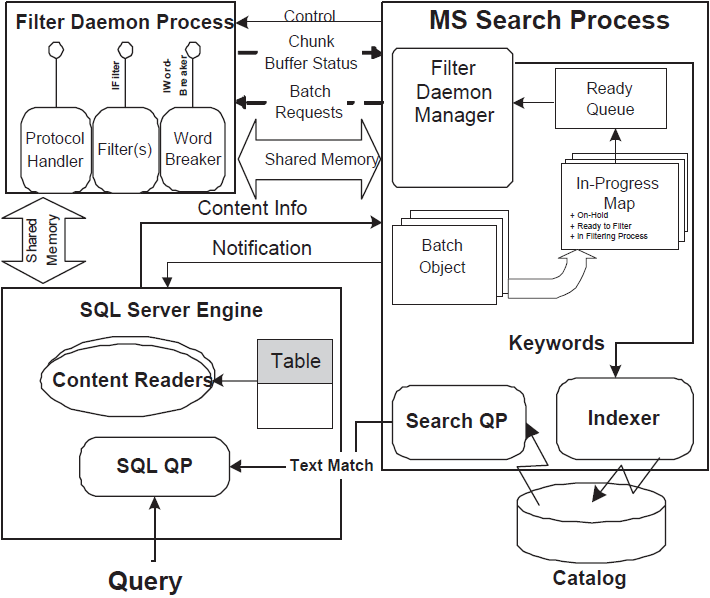
\includegraphics[width=0.9\textwidth]{sql_search_architecture.png}
    \\
    \cite[Source:][p. 8]{hamilton_microsoft_2001}
\end{figure}
\textbf{Word breakers} split the chunks into keywords and additionally provide alternative keywords and the corresponding position in the text. Word breakers can recognize human languages and on \ac{SQL} Server several word breakers for different languages are installed by default. The generated keywords and metadata are passed on to the \ac{MS} Search process, which processes the data with an indexer.\\
The \textbf{indexer} generates an inverted keyword list with a batch containing all keywords of one or more items. These indexes are compressed to use memory efficiently, this may lead to high costs for updates of these indexes. Therefore a stack of indexes is maintained. New documents first create their small indexes, which are regularly merged into a larger index, which in turn is merged into the base index. This stack can be deeper than three, but the concept remains and allows a strongly compressed index without driving the update costs too high. If a keyword is searched, all indexes are accessed, so the depth should still be kept reasonable.\\
A \textbf{query processor} manages the insertion and merge operations and collects statistics on distribution and frequency for ranking purposes and query execution \parencite[cf.][pp. 8-9]{hamilton_microsoft_2001}.
\subsubsection{MS SQL Server Full-Text Query Features}
Full-text indexes can be created on \ac{SQL} Servers with the \ac{DDL} statement \lstinline[language=SQL]$CREATE INDEX$ and can make use of other \ac{SQL} Server utilities; these include backup and restore and attachment of databases. There are three options to create and manage indexes on \ac{SQL} Servers. \textbf{Full Crawl} always rebuilds the whole full-text index by scanning the entire table. \textbf{Incremental Crawl} logs the timestamp of the last re-index and retains changes by storing them in a column. \textbf{Change Tracking} enables a near real-time validity between the full-text index and the table by tracking changes to the indexed data using the \ac{SQL} Server Query Processor \parencite[cf.][p. 9]{hamilton_microsoft_2001}.\\
Full-text search is represented in \ac{SQL} with three possible constructs: \parencite[cf.][p. 9]{hamilton_microsoft_2001}
\begin{enumerate}
    \item Contains Predicate: A contains predicate is true if one of the specified columns contains terms that satisfy the specified search condition. E.g. \lstinline[language=SQL]$Contains(author, ('Ag* or "Marc Miller"'))$ will match entries where the column author contains words like 'Ag', 'Agatha', or 'Marc Miller'.
    \item Freetext Predicate: Freetext predicates are true if one of the specified columns contains terms that stem from the terms in the specified search condition. E.g. \lstinline[language=SQL]$Freetext(content, 'fishing')$ will match entries where content contains words like 'fishing', 'fish', or 'fisher'.
    \item ContainsTable and FreetextTable: ContainsTable and FreetextTable are functions that match entries similar to their corresponding function, but additionally return multiple matches including a ranking for each entry and the entire corpus.
\end{enumerate}
The search conditions of these constructs can be of various types to find the intended results: \parencite[cf.][p. 9]{hamilton_microsoft_2001}
\begin{enumerate}
    \item Keyword, phrase, prefix: E.g. 'fishing', 'Marc Miller', 'Ag*'
    \item Inflections and Thesaurus: E.g. \lstinline[language=SQL]$Contains(*, 'FORMSOF(INFLECTIONAL, fishing) AND FORMSOF(THESAURUS, boat)')$ will find all entries containing words that stem from 'fishing' and all words sharing the meaning with 'boat' (Thesaurus support).
    \item Weighted terms: Keywords and phrases can be assigned a relative weight to impact the rank of entries. E.g. \lstinline[language=SQL]$ContainsTable(*, 'ISABOUT(generator weight (.7), full-text weight (.3))')$ will rank entries higher in the result corpus which mention 'generator' over 'full-text'.
    \item Proximity: E.g. \lstinline[language=SQL]$Contains(*, 'corn NEAR salad')$ contains the proximity term 'NEAR' to match entries where 'corn' appears close to 'salad'.
    \item Composition: E.g. \lstinline[language=SQL]$Contains(*, 'full-text AND NOT database')$ uses two search query components that are composed using a term like 'AND', 'OR', or 'AND NOT'.
\end{enumerate}
